% !TeX spellcheck = en_US
% !TeX encoding = utf8
% !TeX program = xelatex
% !BIB program = bibtex

\documentclass[12pt,notes,mathserif]{beamer}
% \documentclass[draft]{beamer}	
\usetheme{Singapore}
% \usetheme{Hannover}
%\usepackage{pgfpages}
%\setbeameroption{show notes on second screen}

\usepackage[british]{babel}
\usepackage{graphicx,hyperref,url}
\usepackage{mmstyles,bm,ulem}

\usepackage{listings}
\usefonttheme[onlymath]{serif}
\usepackage{fontspec}
\usepackage{xeCJK}
% \setCJKfamilyfont{hei}{SimHei}
% \setCJKmainfont[BoldFont=Arial, ItalicFont=Arial]{Arial}
% \pgfdeclareimage[width=\paperwidth,height=\paperheight]{bg}{background}
% \setbeamertemplate{background}{\pgfuseimage{bg}}
%% columns
\newcommand{\begincols}[1]{\begin{column}{#1}}
\newcommand{\stopcols}{\end{column}}
\newcommand{\pp}[2]{\frac{\partial #1}{\partial #2}}
% \usepackage[backend=biber]{biblatex}
% \bibliography{./ref.bib}
%\addbibresource{ref.bib}
\usepackage{indentfirst}
\usepackage{longtable}
\usepackage{float}
\usepackage{rotating}
\usepackage{subfigure}
\usepackage{tabu}
\usepackage{amsmath}
\usepackage{amssymb}
\usepackage{setspace}
\usepackage{amsfonts}
\usepackage{appendix}
\usepackage{listings}
\usepackage{xcolor}
\usepackage{colortbl}
\usepackage{geometry}
% \setCJKfamilyfont{cjkhwxk}{SimSun}
% \newcommand*{\cjkhwxk}{\CJKfamily{cjkhwxk}}
%\newfontfamily{\consolas}{Consolas}
%\newfontfamily{\monaco}{Monaco}
%\setmonofont[Mapping={}]{Consolas}	%英文引号之类的正常显示,相当于设置英文字体
%\setsansfont{Consolas} %设置英文字体 Monaco, Consolas,  Fantasque Sans Mono
% \setmainfont{Times New Roman}
% \newfontfamily{\consolas}{Times New Roman}
% \newfontfamily{\monaco}{Arial}
% \setCJKmainfont{Times New Roman}
%\setmainfont{MONACO.TTF}
%\setsansfont{MONACO.TTF}
\newcommand{\verylarge}{\fontsize{60pt}{\baselineskip}\selectfont}  
\newcommand{\chuhao}{\fontsize{44.9pt}{\baselineskip}\selectfont}  
\newcommand{\xiaochu}{\fontsize{38.5pt}{\baselineskip}\selectfont}  
\newcommand{\yihao}{\fontsize{27.8pt}{\baselineskip}\selectfont}  
\newcommand{\xiaoyi}{\fontsize{25.7pt}{\baselineskip}\selectfont}  
\newcommand{\erhao}{\fontsize{23.5pt}{\baselineskip}\selectfont}  
\newcommand{\xiaoerhao}{\fontsize{19.3pt}{\baselineskip}\selectfont} 
\newcommand{\sihao}{\fontsize{14pt}{\baselineskip}\selectfont}      % 字号设置  
\newcommand{\xiaosihao}{\fontsize{12pt}{\baselineskip}\selectfont}  % 字号设置  
\newcommand{\wuhao}{\fontsize{10.5pt}{\baselineskip}\selectfont}    % 字号设置  
\newcommand{\xiaowuhao}{\fontsize{9pt}{\baselineskip}\selectfont}   % 字号设置  
\newcommand{\liuhao}{\fontsize{7.875pt}{\baselineskip}\selectfont}  % 字号设置  
\newcommand{\qihao}{\fontsize{5.25pt}{\baselineskip}\selectfont}    % 字号设置 

\graphicspath{{./fig/}}

% \setbeamertemplate{footnote}{%
%   \hangpara{2em}{1}%
%   \makebox[2em][l]{\insertfootnotemark}\footnotesize\insertfootnotetext\par%
% }

\definecolor{cred}{rgb}{0.6,0,0}
\definecolor{cgreen}{rgb}{0.25,0.5,0.35}
\definecolor{cpurple}{rgb}{0.5,0,0.35}
\definecolor{cdocblue}{rgb}{0.25,0.35,0.75}
\definecolor{cdark}{rgb}{0.95,1.0,1.0}
\lstset{
	language=R,
	numbers=left,
	numberstyle=\tiny\color{black},
	keywordstyle=\color{cpurple}\consolas,
	commentstyle=\color{cgreen}\consolas,
	stringstyle=\color{cred}\consolas,
	frame=single,
	escapeinside=``,
	xleftmargin=1em,
	xrightmargin=1em, 
	backgroundcolor=\color{cdark},
	aboveskip=1em,
	breaklines=true,
	tabsize=3
} 

\providecommand{\tightlist}{%
	\setlength{\itemsep}{0pt}\setlength{\parskip}{0pt}}

	
\title{Basic Feedforward Network}

\author[YingmingLi]{Yingming Li \\ yingming@zju.edu.cn}

\institute[DSERC, ZJU]{Data Science \& Engineering Research Center, ZJU}

\date[\today]{\today}

\begin{document}

\AtBeginSection[]
{
	\begin{frame}
		\frametitle{Outline}
		\tableofcontents[currentsection]
	\end{frame}
}

% \AtBeginSubsection[2-]
% {
%    \begin{frame}
%        \frametitle{Outline}
%        \tableofcontents[currentsection]
%    \end{frame}
% }
\begin{frame}[c]
	\titlepage
	Adapted from Prof. Fuxin Li's slides. 
\end{frame}

\section{}\label{section}

\begin{frame}{Linear Classifier and the Perceptron Algorithm}

\begin{itemize}
\item
  \(f(x)=\sigma(w^T{x}+b)\)
\item
  Note: vector or matrix can be judged by context, e.g., here \(w\) and
  \(x\) is vector.
\item
  \(\sigma\): Sigmoid function \(\sigma(x)=\frac{1}{1+e^{-x}}\)
\item
  The connection to logistic regression:

  \begin{itemize}
  \tightlist
  \item
    Assume binomial distribution with parameter \(\hat{p}\)
  \item
    Assume the logit transform is linear:
    \[\log\frac{\hat{p}}{1-\hat{p}}=w^{{T}}x+b\]
    \[\Rightarrow\ \hat{p}=\sigma(f(x))\]
  \end{itemize}
\end{itemize}

\end{frame}

\begin{frame}{Maximum Log-Likelihood}

\begin{itemize}
\tightlist
\item
  MLE of the binomial likelihood:
\end{itemize}

\[\sum_{i=1} ^{n} y_i^* \log \hat{p} + (1-{y}_{i}^{*})\log(1-\hat{p})\]

where \({y}_{i}^{*}\in \{0,1\} =\frac{1+y_{i}}{2}\)

\[\log\hat{p}=-\log(1+e^{-f(x)})\] \[\log(1-\hat{p})=-\log(1+e^{f(x)})\]
\[{y}_{{i}}^{*}\log\hat{p}+(1-{y}_{i}^{*})\log(1-\hat{p})=-\log(1+e^{-yf(x)})\]

\end{frame}

\begin{frame}{Gradient descent optimization}

\begin{itemize}
\tightlist
\item
  Optimize \(w, b\) with gradient descent
\end{itemize}

\[\min_{w,b}\sum_{i}\log(1+e^{-y_{i}(w^{{T}}x_{i}+b)})\]

\[\nabla w=\sum_{i}\frac{-{y}_{i}e^{-y_{i}(w^{{T}}x_{i}+b)}}{1+e^{-y_{i}(w^{{T}}x_{i}+b)}}x_{i}=\sum_{i}-{y}_{i}^{*}(1-\hat{p}(x_{i}))-(1-{y}_{i}^{*})\hat{p}(x_{i})x_{i}\]

\[\nabla b=\sum_{i}\frac{-{y}_{i}e^{-y_{i}(w^{{T}}x_{i}+b)}}{1+e^{-y_{i}(w^{{T}}x_{i}+b)}}\]

\end{frame}

\begin{frame}{XOR problem and linear classifier}

\begin{itemize}
\item
  4 points: \({X}=[(-1,-1),\ (-1,1),\ (1,-1),\ (1,1)]\)
\item
  \(Y=[-1, 1, 1, -1]\)
\item
  Try using binomial \(\log\)-likelihood loss: \[
  \min_{w}\sum_{i}\log(1+e^{-y_{i}(w^{{T}}x_{i}+ b)})
  \]
\item
  Gradient:
  \[\nabla w=\sum_{i}\frac{-{y}_{i}e^{-y_{i}(w^{{T}}x_{i}+b)}}{1+e^{-{y}i(w^{{T}}x_{i}+b)}}x_{i}\]
  \[\nabla b=\sum_{i}\frac{-{y}_{i}e^{-y_{i}(w^{{T}}x_{i}+b)}}{1+e^{-\mathcal{y}i(w^{{T}}x_{i}+b)}}\]
\item
  Try \(w=0, b=0\), what do you see?
\end{itemize}

\end{frame}

\begin{frame}{With 1 hidden layer}

\begin{columns}
    \begincols{.5\textwidth}
        \begin{itemize}
            \item A hidden layer makes a nonlinear classifier
            $$
            f(x)=w^{{T}}g(W^{{T}}x+c)+b
            $$
            \item  ${g}$ needs to be nonlinear
            \item Sigmoid: $\sigma(x)=1/(1+e^{-x})$
            \item RELU: $g({x})=\max(0,{x})$
        \end{itemize}
    \stopcols
    \begincols{.5\textwidth}
    \begin{center}
        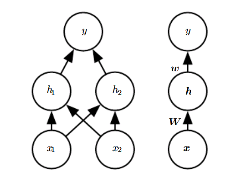
\includegraphics[width=\textwidth]{2018-04-15-13-08-28.png}
    \end{center}
    \stopcols
        
\end{columns}

\end{frame}

\begin{frame}{Taking gradient}

\[
\min_{W,w}E(f)=\sum_{i}L(f(x_{i}),y_{i})
\] \[
f(x)=w^{T}g(W^{T}x+c)+b
\]

\begin{itemize}
\item
  What is \(\frac{\partial E}{\partial W}\) ?
\item
  Consider chain rule: \(\frac{dz}{dx}=\frac{dz}{dy}\frac{dy}{dx}\)
\end{itemize}

\end{frame}

\begin{frame}{Note: Vectorized Computations}

\begin{itemize}
\tightlist
\item
  The computations performed by a network. \[z_i = \sum_{i} W_{ij} x_j\]
  \[h_i=\sigma(z_i)\] \[y=\sum_i v_i h_i\]
\item
  Write them in terms of matrix and vector operations.
\item
  Note: judge vector or matrix by context \[z=Wx\] \[h=\sigma(z)\]
  \[y=v^T h\]
\item
  Where \(\sigma(v)\) denote the logistic sigma function applied
  elementwise to a vector \(v\). Let \(W\) be a matrix where the
  \((i,j)\) entry is the weight from visible unit \(j\) to hidden unit
  \(i\).
\end{itemize}

\end{frame}

\begin{frame}{Backpropagation}

\begin{itemize}
\tightlist
\item
  Save the gradients and the gradient products that have already been
  computed to avoid computing multiple times
\item
  In a multiple layer network(Ignore constant terms)\\

  \begin{center}
  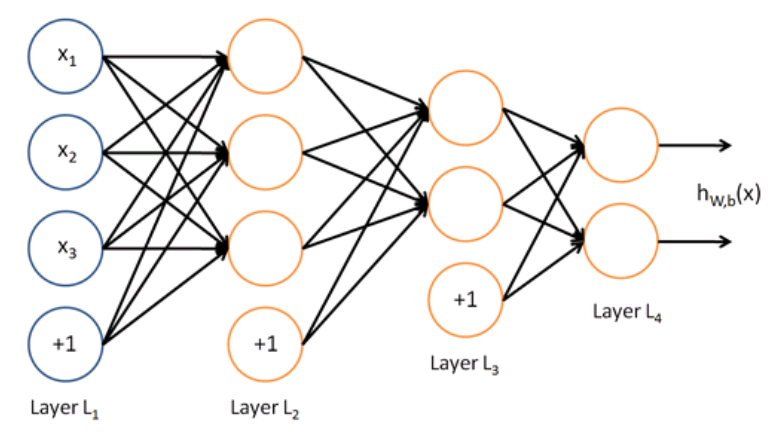
\includegraphics[width=\textwidth]{2018-04-15-13-09-15.png}
  \end{center}
\end{itemize}

\textbackslash{}end\{columns\}

\end{frame}

\begin{frame}{Backpropagation}

\begin{itemize}
\tightlist
\item
  Save the gradients and the gradient products that have already been
  computed to avoid computing multiple times
\item
  In a multiple layer network(Ignore constant terms)\\
  \[f(x)=w_{n}^{T}g (W_{n-1}^{T}g(W_{n-2}^{T}g\ (W_{1}^{T}g(x)))))\] \[
      \frac{\partial E}{\partial W_{k}}=\frac{\partial E}{\partial f_{k}}g(f_{k-1}(x))
      =\frac{\partial E}{\partial f_{k+1}}\frac{\partial f_{k+1}}{\partial f_{k}}g(f_{k-1}(x))
      \]
\item
  Define: \(f_{k}(x)=w_{k}^{T}g(f_{k-1}(x)), f_{0}(x)=x\)
\end{itemize}

\end{frame}

\begin{frame}{Modules}

\begin{itemize}
\tightlist
\item
  Each layer can be seen as a module
\item
  Given input, return

  \begin{columns}
  \begincols{.6\textwidth}
  \begin{itemize}
      \item \begin{itemize}
          \item  Output $f_{a}(x)$
          \item   Network gradient $\frac{\partial f_{a}}{\partial x}$
          \item  Gradient of module parameters $\frac{\partial f_{a}}{\partial w_a}$
      \end{itemize}
  \end{itemize}
  \stopcols
  \begincols{.4\textwidth}
  \begin{center}
      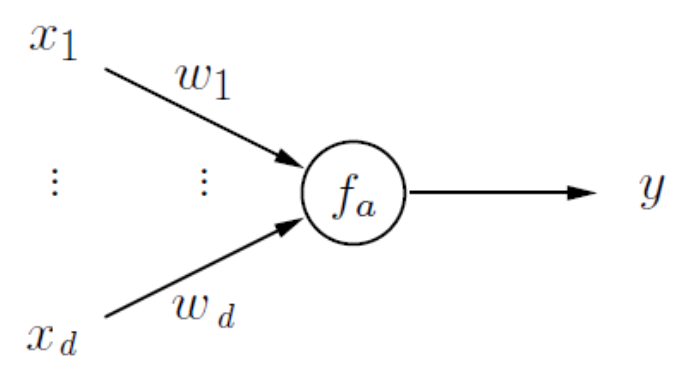
\includegraphics[width=\textwidth]{2018-04-15-13-09-43.png}
  \end{center}
  \stopcols
  \end{columns}
\item
  During backprop, propagate/update

  \begin{itemize}
  \tightlist
  \item
    Backpropagated gradient \(\frac{\partial E}{\partial f_{a}}\)
    \[\frac{\partial E}{\partial W_{k}}=\frac{\partial E}{\partial f_{k}} g(f_{k-1}( x))=\frac{\partial E}{\partial f_{k + 1} }\pp{f_{k+1}}{f_k}g(f_{k-1}(x))\]
  \item
    Three term above are respectively Backprop signal; Network Gradient;
    gradient of parameters
  \item
    Note:
    \(\frac{\partial E}{\partial f_{k}}=\pp{E}{f_{k+1}} \pp{f_{k+1}}{{f_k}}\)
  \end{itemize}
\end{itemize}

\end{frame}

\begin{frame}{Multiple Inputs and Multiple Outputs}

\[\frac{\partial E}{\partial f_{k-1}}=\pp{E}{f_{k+1}}\pp{f_{k+1}}{f_{k_1}}\pp{f_{k_1}}{f_{k-1}}+\pp{E}{f_{k+1}} \pp{f_{k+1}}{f_{k_2}}\pp{f_{k_2}}{f_{k-1}}\]

\begin{center}
    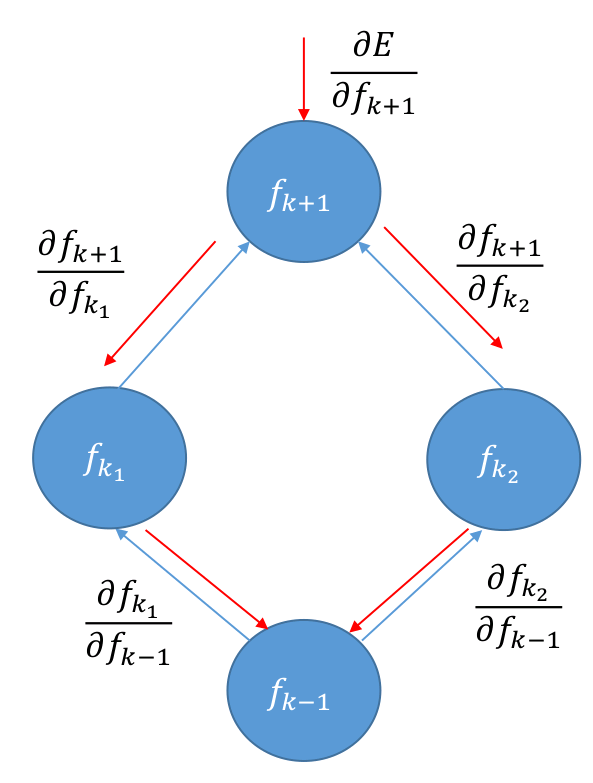
\includegraphics[width=.4\textwidth]{2018-04-15-13-10-08.png}
\end{center}

\end{frame}

\begin{frame}{Different DAG structures}

\begin{itemize}
\tightlist
\item
  The backpropation algorithm would work for any DAGs
\item
  So one can imagine different architectures than the plain layerwise
  one
\end{itemize}

\begin{center}
    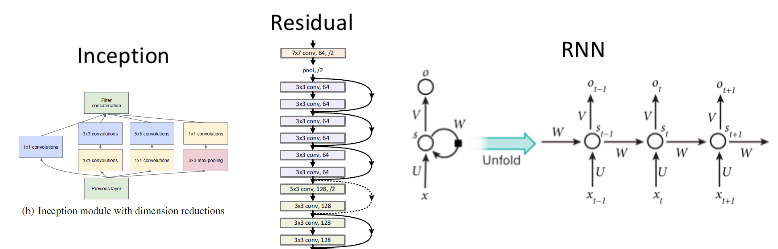
\includegraphics[width=.9\textwidth]{2018-04-14-00-19-13.png}
\end{center}

\end{frame}

\begin{frame}{Loss functions}

\begin{itemize}
\tightlist
\item
  Regression:

  \begin{itemize}
  \tightlist
  \item
    Least squares \(L(f)=(f(x)-y)^{2}\)
  \item
    L1 loss \(L(f)=|f(x)-y|\)
  \item
    Huber loss
    \[L({f})=\begin{cases} \frac{1}{2} (f(x)-y)^2 & , |f(x)-y| \le \delta \\ \delta (|f(x)-y| -\frac{1}{2} \delta ) & \textrm{, otherwise} \end{cases}\]
  \end{itemize}
\end{itemize}

\begin{center}
    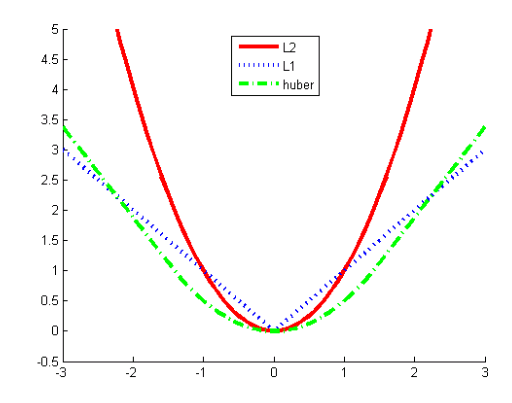
\includegraphics[width=.42\textwidth]{2018-04-15-13-10-18.png}
\end{center}

\end{frame}

\begin{frame}{Loss functions}

\begin{itemize}
\tightlist
\item
  Regression:

  \begin{itemize}
  \tightlist
  \item
    Least squares \(L(f)=(f(x)-y)^{2}\)
  \item
    L1 loss \(L(f)=|f(x)-y|\)
  \item
    Huber loss
    \[L({f})=\begin{cases} \frac{1}{2} (f(x)-y)^2 & , |f(x)-y| \le \delta \\ \delta (|f(x)-y| -\frac{1}{2} \delta ) & \textrm{, otherwise} \end{cases}\]
  \end{itemize}
\item
  Binary Classification

  \begin{itemize}
  \tightlist
  \item
    Hinge loss \(L(f)=\max(1-yf(x), 0)\)
  \item
    Binomial log-likelihood \(L(f)=\ln(1+\exp(-2yf(x))\)
  \item
    Cross-entropy
    \(L(f)=-y^{*}\ln \sigma(f)-(1-y^{*})\ln(1- \sigma(f))\) ,
  \item
    \(y^{*}=(y+1)/2\)
  \end{itemize}
\end{itemize}

\end{frame}

\begin{frame}{Multi-class: Softmax layer}

\begin{itemize}
\tightlist
\item
  Multi-class logistic loss function
\end{itemize}

\[P(y=j|x)=\frac{e^{x^Tw_j}}{\sum_{k=1}{K}e^{x^Tw_k}}\]

\begin{itemize}
\tightlist
\item
  \{\rm Log\}-likelihood:
\item
  Loss function is minus \(\log\)-likelihood \[
  -\log P(y=j|x)=-x^{T}w_{\dot{j}}+\log\sum_{k}e^{x^{T}w_{k}}
  \]
\end{itemize}

\end{frame}

\begin{frame}{Subgradients}

\begin{itemize}
\tightlist
\item
  What if the function is non-differentiable?
\item
  Subgradients:

  \begin{itemize}
  \tightlist
  \item
    For convex \(f(x)\) at \(x_{0}\):\\
  \item
    If for any \(y\) \[f(y)\geq f(x)+g^T(y-x)\]
  \item
    \(g\) is called a subgradient
  \end{itemize}
\item
  Subdifferential: \(\partial f\): set of all subgradients
\item
  Optimality condition: \(0\in\partial f\)
\end{itemize}

\begin{center}
    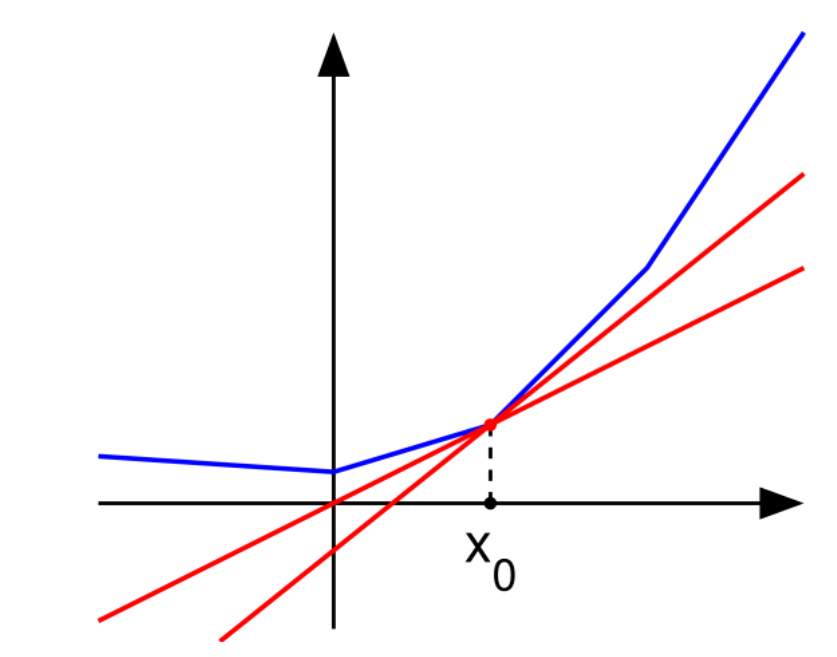
\includegraphics[width=.375\textwidth]{2018-04-15-13-10-32.png}
\end{center}

\end{frame}

\begin{frame}{The RELU unit}

\begin{itemize}
\tightlist
\item
  \(f(x)=\max(x,0)\)
\item
  Convex
\item
  Non-differentiable
\item
  Subgradient:
  \(\frac{\partial f}{\partial x}=\begin{cases} 1 &,x>0 \\ [0,1]&,x=0 \\ 0&,x<0 \end{cases}\)
\end{itemize}

\begin{center}
    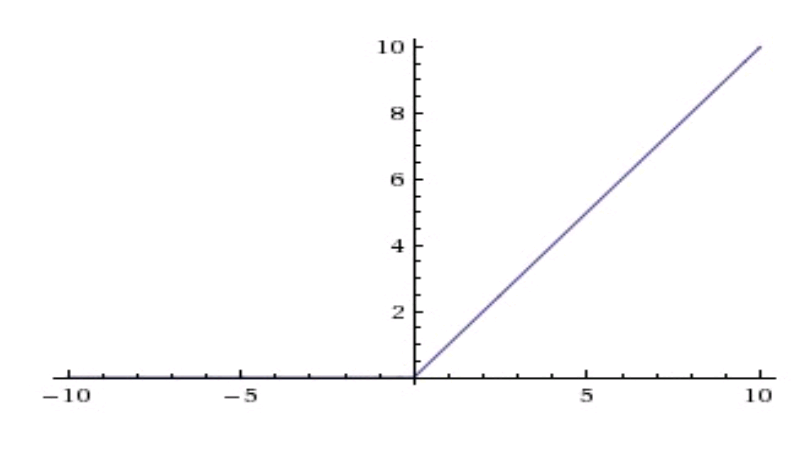
\includegraphics[width=.5\textwidth]{2018-04-15-13-10-48.png}
\end{center}

\end{frame}

\begin{frame}{Subgradient descent}

\begin{itemize}
\tightlist
\item
  Similar to gradient descent \[x^{(k+1)}=x^{(k)}-\alpha_k g^{(k)}\]
\item
  Step size rules:

  \begin{itemize}
  \tightlist
  \item
    Constant step size: \(\alpha_k = \alpha\)
  \item
    Square summable:
    \(\alpha_k\ge 0, \sum_{k=1}^{\infty} \alpha_k^2 < \infty, \sum_{k=1}^{\infty}\alpha_k =\infty\)
  \item
    Usually, a large constant that drops slowly after a long while .
    e.g. \(\frac{100}{100+k}\)
  \end{itemize}
\end{itemize}

\end{frame}

\begin{frame}{Universal Approximation Theorems}

\begin{itemize}
\tightlist
\item
  Many universal approximation theorems proved in the \(90s\)
\item
  Simple statement: for every continuous function, there exist a
  function that can be approximated by a 1-hidden layer neural network
  with arbitrarily high precision
\end{itemize}

\begin{center}
    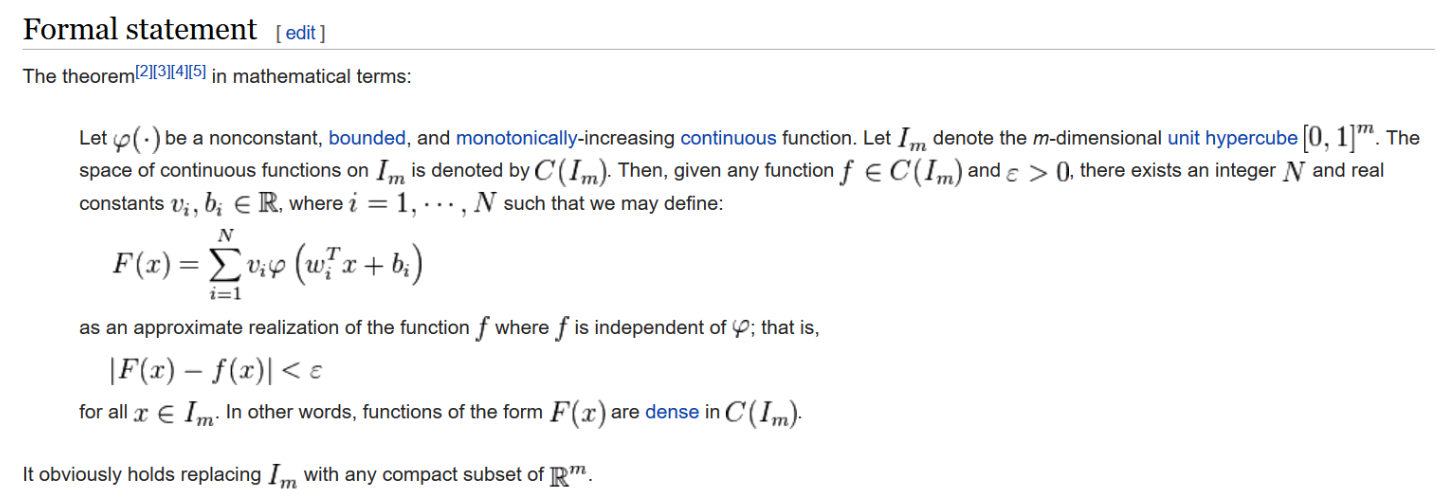
\includegraphics[width=\textwidth]{2018-04-15-13-11-16.png}
\end{center}

\end{frame}

\begin{frame}{Universal Approximation Theorems}

\begin{itemize}
\tightlist
\item
  The approximation does not need many units if the function is kinda
  nice. Let \[C_{f}=\int_{R_{d}}||\omega|||\tilde{f}(\omega)|d\omega\]
\item
  Then for a 1-hidden layer neural network with \(n\) hidden nodes, we
  have for a finite ball with radius \(r\), \[
  \int_{B_{r}}(f(x)-f_{n}(x))^{2}d \mu(x)\leq\frac{4r^{2}C_{f}^{2}}{n}
  \]
\end{itemize}

\end{frame}

\begin{frame}
	\begin{center}
		\chuhao Thank you!  
	\end{center}
\end{frame}
\end{document}
